\section{Arjun Yuda Firwanda}
\subsection{Teori}
\subsubsection{Apa itu fungsi library matplotlib}
\hfill \break
Matplotlib pada python merupakan sebuah library plotting python yang menghasilkan sebuah gambar.

\subsubsection{Jelaskan langkah-langkah membuat sumbu X dan Y di matplotlib}
\hfill \break
Berikut contoh membuat sumbu x dan y yang menggunakan list untuk mempermudah penyimpanan nilai setiap sumbunya adalah sebagai berikut.
\lstinputlisting[firstline=9, lastline=10]{src/6/1174008/teori/T1174008.py}

\subsubsection{Jelaskan bagaimana perbedaan fungsi dan cara pakai untuk berbagai jenis plot di matplotlib}
\hfill \break
Perbedaan fungsi dari segi bentuk grafik pada hasil kode programnya.
Contoh cara pengguna plot tersebut sebagai berikut.
\begin{itemize}
    \item Line
    Plot Line menggunakan perintah untuk membuat grafik line atau garis sebagai berikut.
    \lstinputlisting[firstline=12, lastline=14]{src/6/1174008/teori/T1174008.py}

    \item Bar
    Plot Bar yang memiliki koordinat x dan koordinat y. Berikut contohnya.
    \lstinputlisting[firstline=16, lastline=25]{src/6/1174008/teori/T1174008.py}

    \item Histogram
    Plot Histogram akan menampilkan grafik frekuensi data berdasarkan kode program yang dijalankan.
    Berikut adalah contohnya.
    \lstinputlisting[firstline=27, lastline=34]{src/6/1174008/teori/T1174008.py}

    \item Scatter
    Plot Scatter merupakan diagram yang menghasilkan diagram titik.
    Berikut contoh plot scatter.
    \lstinputlisting[firstline=36, lastline=49]{src/6/1174008/teori/T1174008.py}

    \item Stack plot
    Plot Stack Plot digunakan untuk membuat diagram seperti halnya plot line yang membedakannya dari hal warna. Jadi diagram yang dihasilkan terdapat warna.
    Berikut Contoh penggunaannya.
    \lstinputlisting[firstline=82, lastline=92]{src/6/1174008/teori/T1174008.py}
\end{itemize}

\subsubsection{Jelaskan bagaimana cara menggunakan legend dan label serta kaitannya dengan fungsi tersebut}
\hfill \break
Untuk menggunakan legend dan label bisa di lihat dibawah ini
\lstinputlisting[firstline=20, lastline=22]{src/6/1174008/teori/T1174008.py}
Penggunaan legend pada python untuk mempermudah dalam membaca grafik. Legend berisikan info grafik yang ditampilkan meliputi bentuk, nama, warna. Legend juga digunakan untuk membedakan titik x dan titik y.

\subsubsection{Jelaskan apa fungsi dari subplot di matplotlib, dan bagaimana cara kerja dari fungsi subplot, sertakan ilustrasi dan gambar sendiri dan apa parameternya jika ingin menggambar plot dengan 9 subplot di dalamnya}
\hfill \break
Fungsi subplot untuk membuat lebih dari satu grafik dalam suatu program.
Berikut contohnya.
\lstinputlisting[firstline=94, lastline=104]{src/6/1174008/teori/T1174008.py}

\subsubsection{Sebutkan semua parameter color yang bisa digunakan}
\hfill \break
Untuk parameter color yang bisa digunakan terdiri dari 2 type warna.
\begin{enumerate}
    \item Tipe Warna RGB atau Red sebagai merah, Green sebagai hijau, Blue sebagai biru.

    \item Tipe warna CMYK atau Cyan sebagai biru muda, Magenta sebagai merah tua, Yellow sebagai kuning, Black sebagai hitam.
\end{enumerate}

\subsubsection{Jelaskan bagaimana cara kerja dari fungsi hist, sertakan ilustrasi dan gambar sendiri}
\hfill \break
Fungsi plot histogram sebagai titik koordinat x dan titik koordinat y, yang masing-masing titik koordinat tidak boleh sama. Contoh titik x ada 5 nilai dan titik y ada 7 nilai.
Contoh dari penggunaan histogram
\lstinputlisting[firstline=27, lastline=34]{src/6/1174008/teori/T1174008.py}

\subsubsection{Jelaskan lebih mendalam tentang parameter dari fungsi pie diantaranya labels, colors, startangle, shadow, explode, autopct}
\hfill \break
Berikut penjelasan tentang parameter yang ada dalam pie.
\begin{itemize}
    \item Label
    Label digunakan untuk mempermudah pembaca dalam membaca diagram pie.

    \item Color
    Color atay=u warna digunakan untuk membedakan warna antar data grafik frekuensi.

    \item Startangle
    Startangle digunakan untuk sudut memulai diagram pie.

    \item Shadow
    Shadow atau bayangan digunakan untuk membuat bayangan dari setiap diagram pie yang menonjol.

    \item Explode
    Explode digunakan untuk mengeluarkan suatu data agar data tersebut terlihat menonjol.

    \item Autopct
    Autopct digunakan sesuai dengan berapa angka dibelakang koma yang kita inginkan.
\end{itemize}

\subsection{Scan Bebas Plagiarisme}
\begin{figure}[H]
\centering
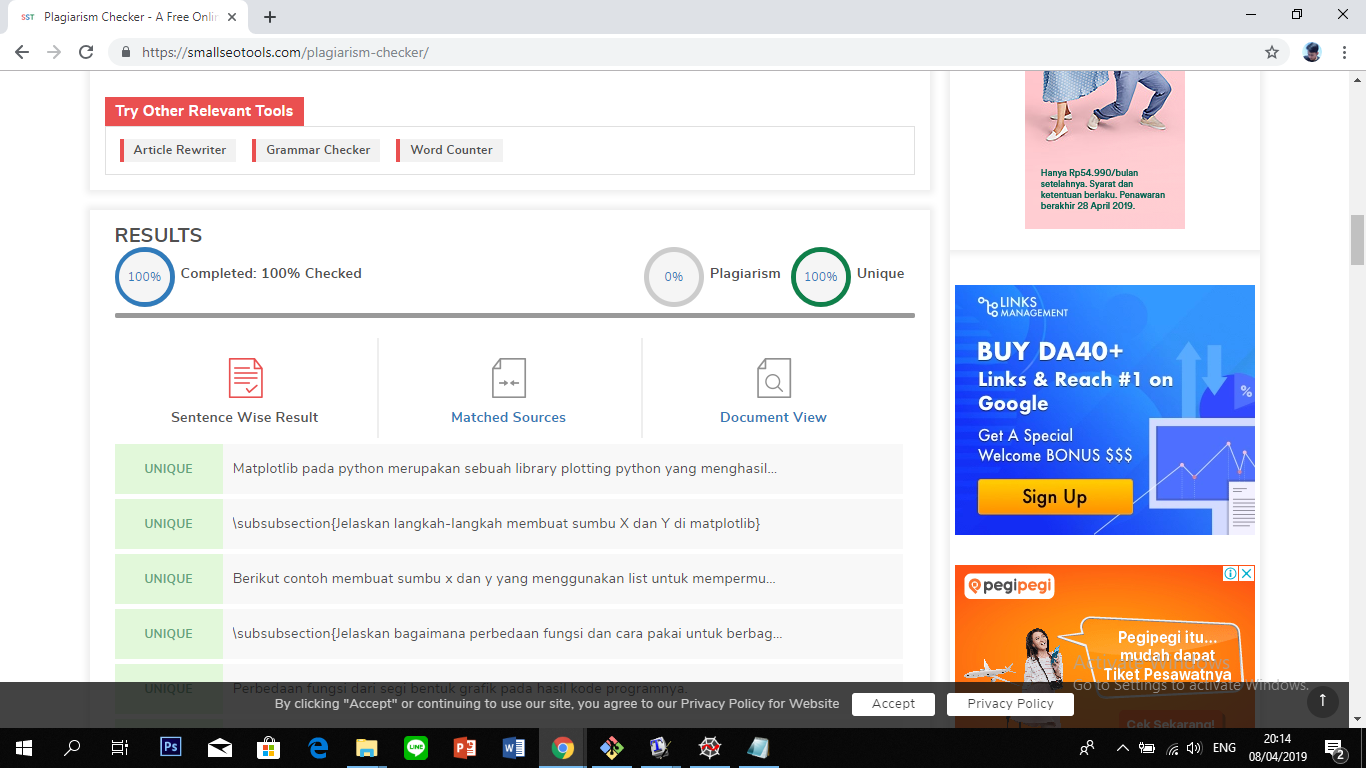
\includegraphics[width=7cm]{figures/6/1174008/bebasplagiarisme.png}
\caption{Scan Bebas Plagiarisme}
\label{Bebas Plagiarisme}
\end{figure}

\subsection{Praktek}
\subsubsection{No 1}
\hfill \break
Dibawah ini merupakan penggunaan subplot dan plot bar.
\lstinputlisting[firstline=8, lastline=28]{src/6/1174008/praktek/p1174008_bar.py}
Dan dibawah ini merupakan cara pemangilannya.
\lstinputlisting[firstline=8, lastline=8]{src/6/1174008/praktek/main_arjun.py}
\lstinputlisting[firstline=13, lastline=13]{src/6/1174008/praktek/main_arjun.py}

\subsubsection{No 2}

\hfill \break

Dibawah ini merupakan penggunaan subplot dan plot scatter.
\lstinputlisting[firstline=8, lastline=28]{src/6/1174008/praktek/p1174008_scatter.py}
Dan dibawah ini merupakan cara pemangilannya.
\lstinputlisting[firstline=9, lastline=9]{src/6/1174008/praktek/main_arjun.py}
\lstinputlisting[firstline=14, lastline=14]{src/6/1174008/praktek/main_arjun.py}

\subsubsection{No 3}

\hfill \break

Dibawah ini merupakan penggunaan subplot dan plot pie.
\lstinputlisting[firstline=8, lastline=50]{src/6/1174008/praktek/p1174008_pie.py}
Dan dibawah ini merupakan cara pemangilannya
\lstinputlisting[firstline=10, lastline=10]{src/6/1174008/praktek/main_arjun.py}
\lstinputlisting[firstline=15, lastline=15]{src/6/1174008/praktek/main_arjun.py}

\subsubsection{No 4}

\hfill \break

Dibawah ini merupakan penggunaan subplot dan plot bar.
\lstinputlisting[firstline=8, lastline=28]{src/6/1174008/praktek/p1174008_plot.py}
Dan dibawah ini merupakan cara pemangilannya
\lstinputlisting[firstline=11, lastline=11]{src/6/1174008/praktek/main_arjun.py}
\lstinputlisting[firstline=16, lastline=16]{src/6/1174008/praktek/main_arjun.py}

\subsection{Penanggan Error}

\hfill \break

Berikut ini merupakan cara penangganan errornya.
\lstinputlisting[firstline=8, lastline=14]{src/6/1174008/praktek/1174008.py}